% \documentclass[11pt,letterpaper]{article}
\documentclass[letterpaper,11.5pt]{scrartcl}
% \documentclass[11pt]{report}
% \documentclass{report}
% \documentclass{book}
\usepackage[bookmarks, hidelinks]{hyperref}
\usepackage{amssymb,amsmath}
% \usepackage{fullpage}
\usepackage{tabulary}
\usepackage{tabularx}
\usepackage{float}
\usepackage[margin=1.00in]{geometry}
% \usepackage[margin=0.90in]{geometry}

\usepackage{caption}
\usepackage{booktabs}
\usepackage{pslatex}
\usepackage{apacite}
\usepackage{subcaption}
\usepackage{pgfplots}
\usepackage{wrapfig}
\usepackage[english]{babel}
\usepackage{lmodern}
\usepackage{setspace}
\doublespace
% \usepackage{url}
\usepackage{bigfoot}
\usepackage[export]{adjustbox}
\setlength\intextsep{0pt}

\usepackage{graphicx}

\title{Some forms of uncertainty may suppress the evolution of social learning}

\author{{}}

\begin{document}
\maketitle

\newcommand{\pisub}[1]{\pi_{\mathrm{#1}}}
\newcommand{\pilow}{\pisub{low}}

\newcommand{\meansl}{\langle s \rangle}


\begin{abstract}

Social learning is essential to survival. It is likely to evolve when it is more
efficient than asocial, trial-and-error learning. The consensus in cultural
evolutionary theory holds that some amount of environmental variability and
uncertainty about the best decisions are necessary for social learning to evolve.
However, current models for the evolution of social learning tend to conflate forms
of uncertainty, and rarely consider different ones in tandem. Moreover, many models
are limited by considering only two possible behaviors and environmental states.
Here we use evolutionary agent-based modeling to improve on these shortcomings. We
model a time-varying environment with dozens of possible behaviors performed by
agents engaging in individual and social learning. We show that ambiguous payoffs,
larger possible decision sets, and shorter agent lifespans sometimes increase social
learning prevalence, as expected. However, we also find that, under some conditions,
these forms of uncertainty can select against social learning.
\end{abstract}

\section{Introduction}

Social learning is essential to human and other species' everyday life and survival.
It allows individuals to solve problems when acquiring information from others is more efficient than learning
on one's own~\cite{Laland2004}. Theory predicts that social
learning should be favored in contexts with greater
uncertainty~\cite{BoydRicherson1985,Henrich1998}, and this prediction has received some empirical support~\cite{McElreath2005,Kendal2018}. 
However, the meaning of the term ``uncertainty'' is not always clear, and often conflates environmental variability, spatial heterogeneity, and ambiguity or uncertainty about payoff structure. 
Moreover, most models of the evolution of social learning ``blackbox'' key 
cognitive learning processes that underlie it~\cite{Heyes2016}. 

In this paper we use agent-based modeling to compare the effect of
different sources of uncertainty on social learning
by ``unblackboxing'' typically abstracted-out model components 
of environmental variability, payoff structures and
agent life histories, and  learning mechanisms. ``Uncertainty''  
means variability where the probabilistic structure is unknown. %cannot be learned.
Uncertainty increases when payoffs are more similar across behaviors, when
environmental variability increases, when the number of possible behaviors
increases, and when lifespan decreases.  In this paper we show that more ambiguous
payoff structures and shorter lifespans sometimes do lead to greater reliance on
social learning---however, we also identify and explain cases where greater
uncertainty leads to less social learning due to the possibility that social
information is misleading.  We thus conclude that many predictions made by previous
models of the evolution of social learning are likely overgeneralized.
%~\cite{Yarkoni2021}. 

\subsection{Social Learning}

Social learning, as we consider it here, occurs whenever an individual acquires a behavior by observing another individual. This need not require explicit instruction, and is, in fact, widespread across a broad range of nonhuman 
taxa~\cite{Kendal2018,Allen2019}. Importantly, social information can be inherited both
from parents --- i.e., via \emph{vertical transmission} like genetic information --- and
from others in the same generation --- i.e., via \emph{horizontal transmission}
\cite{CavalliFeldman1981}. The joint action of vertical and horizontal transmission
gives rise to qualitatively different evolutionary dynamics. For example,
inter-generational environmental change will affect the adaptive value of genetic
information and vertically-transmitted cultural information more than information
that is horizontally transmitted. We include both horizontal and vertical transmission pathways in our
model. For simplicity, we ignore oblique transmission in which non-parental members
of the previous generation are observed.

Environmental variability has been seen as a key selective force in shaping social learning starting with the first formal models of cultural evolution~\cite{CavalliFeldman1981,BoydRicherson1985}.
Totally stable environments will not favor learning mechanisms because information can become genetically hardwired, while  extreme environmental instability will degrade the value
of social learning as information becomes rapidly outdated~\cite{Feldman1996}. This suggests that an intermediate degree of environmental predictability will favor social learning. Strategies can also evolve to mitigate the risks of relying on outdated social information by weighing more heavily information from others who more recently acquired it~\cite{Rendell2010}.

Uncertainty has also been modelled as arising from other aspects of the environment. 
For example, \citeA{Perreault2012} vary the ambiguity of the environmental cue individuals get through individual learning about the state of the world. Perhaps not surprisingly, the more ambiguous the asocial information, the greater the selection for weighing social information heavily. Alternatively, uncertainty about the optimal behavior has been modelled by increasing the number of cultural traits to choose from. 

Empirical research supports some of these theoretical predictions. Organisms flexibly use social learning as a function of the ambiguity of the environmental cue and of other environmental features that are often subsumed under the rubric of ``uncertainty.''
While some studies explicitly impose a cost whenever participants use asocial
information \cite{Morgan2012,Atkisson2012}, 
others allow the costs of each strategy to emerge as a function of task structure and assess its consequences for learning strategies. 
For example, when participants received equivocal private information about the best investment to make in a lab game,
they were more likely to rely on social information to make their choice~\cite{Toelch2013}. 
\citeA{McElreath2005} developed a similar experiment where participants ``pulled'' virtual slot machine arms (often called ``bandits''), each yielding stochastic payoffs. Participants relied more on social learning when the bandits had higher-variance payoffs, and when the highest-paying bandit changed more frequently. 
The number of options to choose between can also increase uncertainty about the optimal choice, and has been shown to increase participants' reliance on social learning \cite{Muthukrishna2016a}. 

Thus existing theoretical work and the empirical evidence seem to support that various forms of uncertainty favor the evolution of social learning. However, uncertain outcomes are operationalized in different ways across models, and any given model tends to focus on only one or two forms of uncertainty at a time. Our agent-based modeling approach enables us to explicitly specify different forms of uncertainty independently in order to understand which of these environmental factors particularly favor the evolution of social learning. Simultaneous modelling also allows us to examine their interaction. We first attempt conceptual replications of previous models' findings, and then examine where they diverge.

\subsection{Research overview}

Computational agents in our model face a problem: every time step they perform
one of several behaviors, with each behavior represented by a ``bandit'' that
pays off 1 or 0 with some probability. One of these behaviors (the optimal
behavior) pays off with a higher probability than all the others.
Agents decide which behavior to 
perform based either on a success-biased observation 
of a peer's behavior (social learning) or based on their own observations (asocial learning).
Agents then update their memory of expected payoffs for each behavior 
when they receive a payoff from their chosen
action. Within this framework we have four mechanisms by which we operationalize 
and vary uncertainty:
(1) the expected payoffs of the optimal behavior and all the rest---when payoffs
are nearly identical, uncertainty in the form of ambiguity increases; (2) the
environmental variability, i.e., the probability that the optimal behavior 
changes between generations; (3) the number of possible behaviors the environment allows---which
behavior is optimal is more uncertain when there are more possibilities; and (4)
 agent lifespan---agents experience fewer learning opportunities and die more uncertain about which behavior
is optimal when their lifespan is shorter. 

The primary outcome measure of our
model is the average difference between the frequency of (horizontal) 
social learning and the frequency of asocial
learning across all agents. If social learning is more prevalent than asocial
learning this suggests that the optimal behavior is more likely found
by copying peers than by trial-and-error search.
Conversely, when asocial learning is more prevalent, this suggests social information
is likely to be misleading. 
When social and asocial learning are 
equally prevalent this means there is no discernible advantage to either, i.e.,
the agents have weak priors on which channel provides more reliable information. 
Each agent has its own social learning frequency that it inherits from its
parent (haploid reproduction) with mutation, so evolution selects for,
or computes~\cite{Smaldino2013}, the optimal
social learning frequency.

Using our model we found that increased uncertainty sometimes
led to increased reliance on social learning, as expected from prior literature. However, we also find cases where increased uncertainty decreased agents' reliance on social learning
due to increased uncertainty that made social information less reliable, thereby
increasing reliance on asocial learning.



\section{Model}

We developed an agent-based model of a society of $N$ individuals who each must decide
which of $B$ behaviors to perform at each time step. Each behavior is a ``bandit'',
a common modelling and experimental approach for representing behaviors with
probabilistic payoffs~\cite{SuttonBartoBook, McElreath2005,Rendell2010,Schulz2019}. %Bandits are like  slot machines in a casino~\ref{fig:behaviorSelection}.
Each behavior $b$ yields a payoff of 1 with probability $\pi_b$ and a payoff of zero
otherwise; $\pi_b$ is therefore also the expected payoff of behavior $b$. Agents must
decide which behavior to perform at each time step. To do this, agents 
use an explore-exploit strategy to sometimes try the most profitable behavior
they know about, and other times try alternatives that may pay off more reliably. 

We operationalized uncertainty in four different ways: 
(1) payoff ambiguity, $A_\pi$, which measures the difference
between the optimal expected payoff behavior $\pisub{high}$ and the expected payoff
of the other behaviors, $\pisub{low}$; 
(2) environmental variability, $u$, the probability the optimal behavior changes from one generation to another; 
(3) the number of possible behaviors, $B$; and 
(4) the lifespan, or time steps per generation, $M$. 

We ran the simulation for $T=1000$ time steps. At
the end of each generation agents reproduce and then die off. 
Those selected to reproduce
pass on their boolean social learning trait, $s$, without mutation,
which specifes whether agents learn socially. We developed a series of
computational analyses where we systematically vary the uncertainty
variables and observe the average prevalence of social learning trait $s$
across agents and trials, which is our primary outcome measure, 
denoted $\langle s \rangle$. 

\subsection{Agents and learning}

In each time step, $N$ agents---autonomous problem solvers---select 
which behavior to perform based on their running tally of mean payoffs for 
each available behavior. %information (Figure~\ref{fig:behaviorSelection}). 
Agents track the mean payoff of each behavior $b$, denoted $\bar\pi_b$, and a \emph{count} of how many times it has performed each behavior, denoted $c_b$. 
Agents' beliefs about mean payoffs are updated from $\bar\pi_b$ to $\bar\pi_b'$ using exponential weighted
averaging, $\bar\pi_b' = \bar\pi_b + \frac{\mathrm{Bandit_b(0, 1)} - \bar\pi_b}{c_b'}$, where
$\mathrm{Bandit}_b(0, 1)$ is 0 or 1 depending on the result of the bandit draw for behavior $b$. 
$\bar\pi_b$ is initialized to 0 for all $b$ at model initialization for
all agents, and after each generation for individual learner agents. Social
learning agents' $\bar\pi_b$ is initialized as that of its teacher selected
through performance-biased oblique learning.

Social learning in this model is oblique, which here means
any agent from the previous generation, including an agent's parent,
could be an agent's teacher. 
Agents learn from exactly one teacher, selected as follows:
First, a learner agent from a new generation selects $N_T$ teachers at random.
The best-performing of the $N_T$ becomes a new agent's teacher, with ties broken
randomly. At the end of each generation, all agents die off with some selected
randomly for reproduction, weighted by accumulated payoffs within the round. 

Following Luce's choice axiom \cite{Luce1959}, an agent using asocial information selects a behavior at random, with the probability of selecting any particular behavior weighted by the softmax function applied to that behavior's observed mean payoff relative to all 
mean payoffs: 
$\Pr(\text{choose behavior }b) = 
  \frac{\exp(\bar\pi_b / \tau) }{ 
\sum_{b=1}^B \exp(\bar\pi_b / \tau)}$.
The softmax method is a biologically plausible model~\cite{Schulz2019} that enables agents to explore alternative behaviors sometimes and exploit the best observed behavior other times.  The parameter $\tau$ specifies
how frequently alternative behaviors are explored---higher $\tau$ means more
frequent exploration. We set $\tau = 0.1$ for all computational analyses 
presented in the main paper. We (WILL) perform(ED) sensitivity analyses 
and found a weak dependence on $\tau$ that does not affect our main conclusions.


\subsection{Modeling uncertainty}

In our model uncertainty is a tunable consequence of four environmental features:
%that structure the behavior of agents.  
% Many factors contribute to the 
% uncertainty involved in both social and asocial learning. 
%We model uncertainty in four distinct ways: 
\begin{enumerate}
    \item We vary the frequency at which the optimal behavior changes, which we call \emph{environmental variability}, $u$. At the start of each generation, with probability $u$, a new behavior is assigned a payoff of $\pisub{high}$ while all other behaviors are assigned a payoff of $\pisub{low}$. Otherwise, the same behavior remains optimal across generations. 
    \item We vary the latent expected payoffs yielded by the bandits. For simplicity,
      we assume that in any given environmental state, there is one optimal behavior that
      yields an expected payoff of $\pisub{high}$, while all other behaviors yield a 
      payoff of $\pisub{low} < \pisub{high}$. 
      The difference between these quantities is the \emph{payoff ambiguity}, 
    \begin{equation}
      A_\pi = 1 - (\pisub{high} - \pisub{low}),
      \label{eq:payoffAmbiguity}
    \end{equation}
    which is maximized when the expected payoffs are close to equal and minimized
    when they differ greatly. For simplicity we will set $\pisub{high} = 0.9$
    for all analyses and vary $\pisub{low}$ in order to vary $A_\pi$.
    \item We vary the total \emph{number of available behaviors}, $B$, which is a
      source of uncertainty since agents are less likely to know which behavior yields high payoffs.  %risk, as it becomes increasingly costly to experiment with alternatives. \cm{is this risk if it reduces variance of outcomes? it sounds like it's just bad for there to be more 0 payoff options}
    \item Finally, we vary number of behavioral events per generation, $M$. This can be viewed as the \emph{effective lifespan} of an agent.  Decreasing this lifespan effectively increases the importance of each event for acquiring payoffs. When lifespans are short ($M$ is small), agents experience greater uncertainty about which behavior is optimal given the fewer learning opportunities.
\end{enumerate}


\subsection{Dynamics and evolution}


\begin{figure}
  \caption{Model dynamics are composed of two major parts: first, agents perform
  behaviors for $M$ time steps in a single generation. Then agents reproduce
  randomly, with more successful agents being more likely to reproduce. Newly
  ``born'' social learner agents use success bias to select and learn from a chosen
  teacher. Then, all agents from the previous generation die off, all new agents
  begin a new generation, and the process continues until 1000 total time steps
  have elapsed. Agents are initialized as ``blank slates''.}
  \centering
    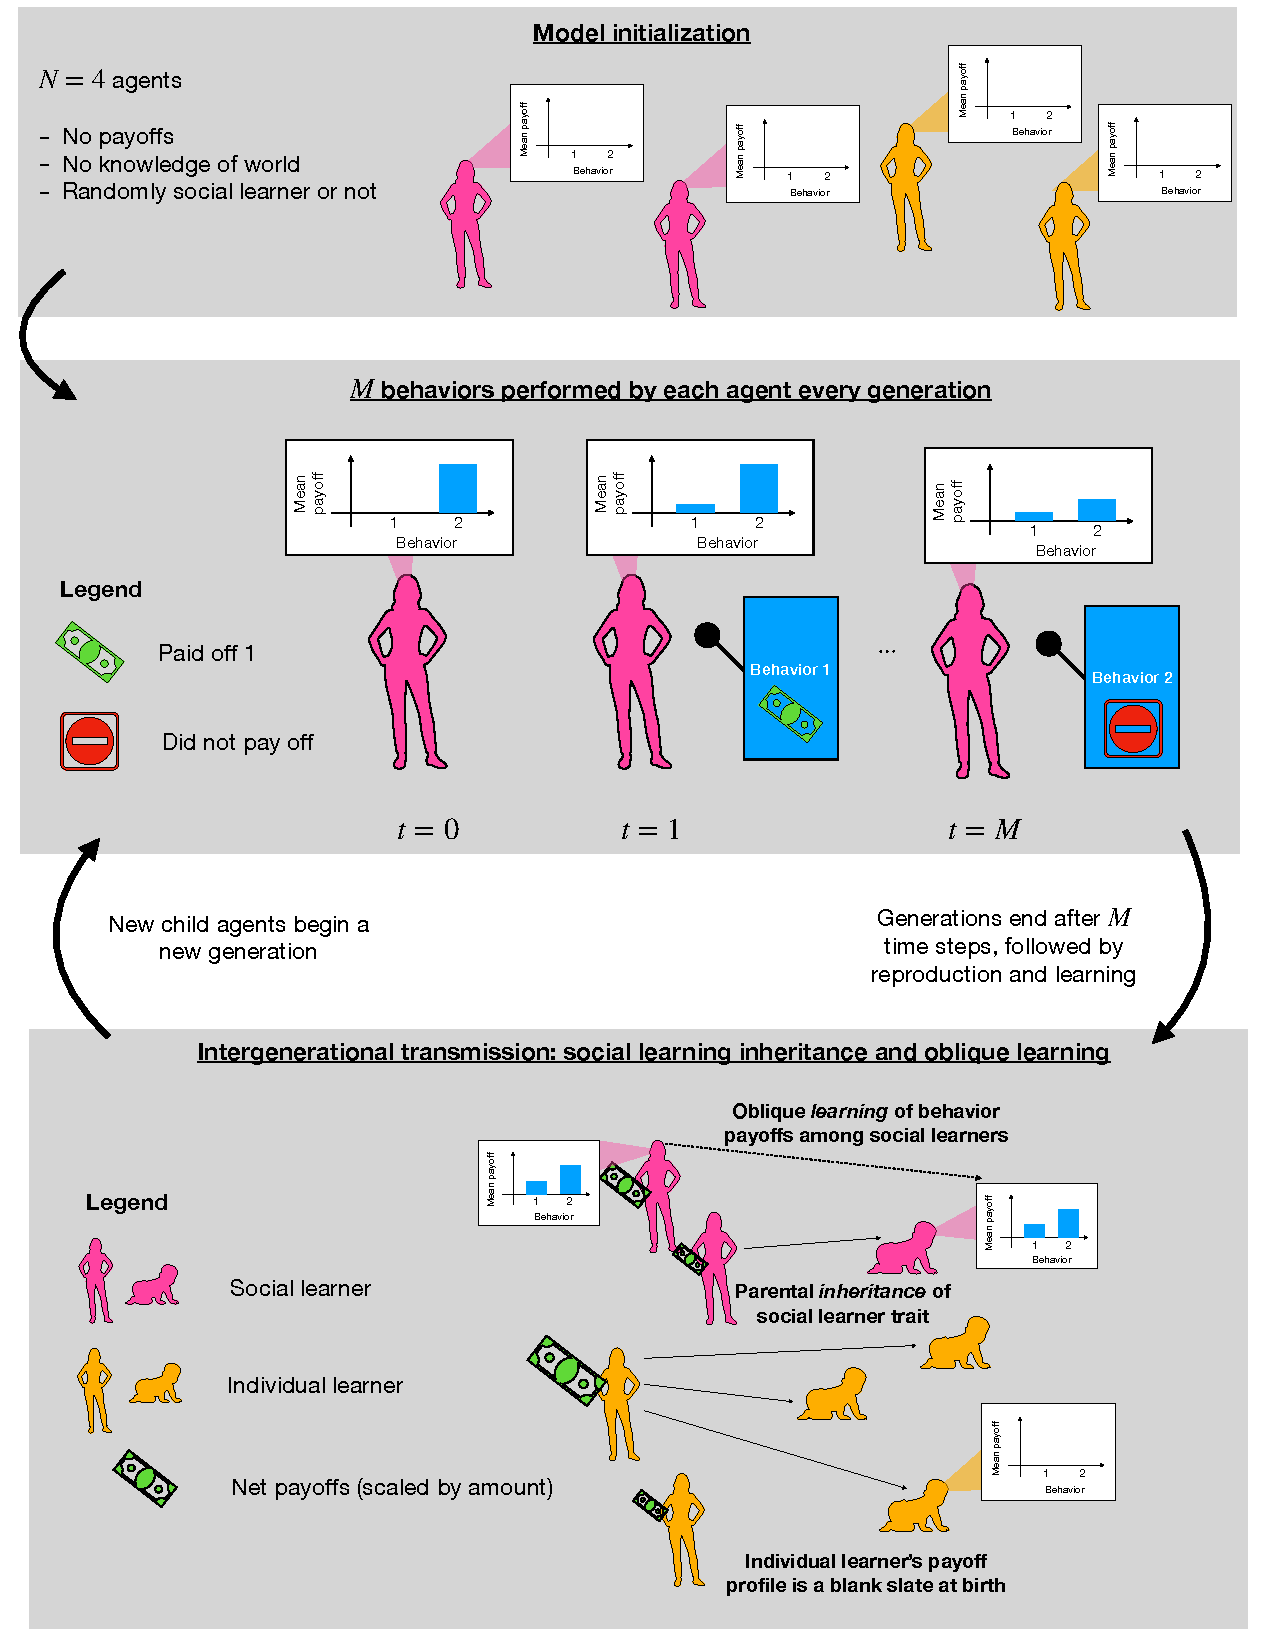
\includegraphics[width=0.9\textwidth]{Figures/IntraInterGenerationalDynamics.pdf}
  \label{fig:IntraInterGenerationalDynamics}
\end{figure}



\subsection{Computational analyses}

We manipulated environmental uncertainty parameters described above, $u$,
$\pisub{low}$, $B$, and $M$, to examine their effects on our
main outcome measure, the prevalence of social learning $s$. For each parameter setting
in our analysis we calculated the average value of $s$ at the final time step
of $T=1000$ across 100 runs for each combination of uncertainty parameter values.

To analyze the effect of various forms of uncertainty on social learning 
prevalence in our Analysis, we initialized several model runs with
different uncertainty parameters $u$, $\pisub{\mathrm{low}}$, $B$,
and $M$. We varied $u \in \{0.0, 0.1, \ldots, 1.0\}$ for each combination of
the following parameters:
$\pisub{low} \in \{0.1, 0.5, 0.8\}$, $B \in \{2, 4, 10\}$, $M \in \{B/2, B, 2B\}$.



\section{Analysis}

\begin{itemize}
  \item 
    To understand how different forms of uncertainty affect social learning evolution
    we systematically varied environmental variables in our model and observed
    corresponding changes in mean social learning prevalence, $\meansl$. We
    confirmed that, in many cases, increased environmental variability $u$ 
    suppresses social learning. However\ldots 


  \item 
    Our analysis confirmed existing theoretical predictions that social learning
    is valuable only when environmental variability $u$ is sufficiently small.
    Because of the central role of $u$, it is set on the x-axis in
    all plots shown in Figure~\ref{fig:results}. 
    The threshold at which social learning stops being strongly selected for
    varies depending on the value of other environmental parameters. 

  \item 
    However, more possible behaviors $B$ ($B=2,4,10$ for the first, second, and
    third column respectively in Figure~\ref{fig:results}) can lead
    social learning to be selected for even for large values of $u$, possibly
    due to the low risk and potentially high reward of learning an accurate
    tally of mean payoffs from the previous generation. 
    Since there are so many behaviors and so
    few observations, softmax weighting will not significantly 
    favor a sub-optimal behavior. However, if one does learn an accurate tally
    then one does have an increased chance of performing the best one.
    \begin{itemize}
      \item 
        (THIS MAKES SENSE, BUT THE EFFECT IS TOO STRONG. WHY SHOULD THERE BE ANY
        SOCIAL LEARNING WHEN U = 1.0?  I THINK SOMETHING IS SLIGHTLY WRONG WITH THE
        MODEL---I'M WORKING ON CHECKING WHAT THAT MIGHT BE)
      \item
        ONE THING TO CHECK IS THE FRACTION DOING THE OPTIMAL BEHAVIOR WHEN
        $u=1$. IF MANY START OUT DOING OPTIMAL, THEN SOMETHING MAY BE WRONG.
    \end{itemize}

  \item 
    $\pilow$ can alter selection selection pressure for or
    against social learning, depending on the number of time steps per generation.
    For instance, when $B=2$, increasing $\pilow$ (i.e. increased uncertainty
    about which behavior is optimal) leads at first to less sharp sigmoid curve, 
    where social learning is less prevalent with increased $\pilow$ when
    $u < 0.5$ and social learning is more prevalent with increased $\pilow$
    when $u > 0.5$. When $\pilow = 0.8$ noise and genetic drift dominate across
    tested values of $B$, with possibly a slight inverse correlation 
    in social learning as $u$ increases. When $B \in \{4,10\}$, increasing
    $\pilow \in \{0.1, 0.5\}$ leads uniformly to increased $\meansl$ over 
    $u$ in those settings.     

  \item
    If $M/B$ has an effect it is mostly to 
    increase reliance on social learning due to social information being of 
    higher quality since teachers would have had more learning opportunities
    for larger $M$. (THERE ARE CASES WHERE THIS IS NOT THE CASE BUT THERE IS 
    STILL TOO MUCH NOISE DUE TO SMALL NTRIALS)

  \item
    Synthesis/analysis conclusion 
    
\end{itemize}




\documentclass[varwidth=true,crop=false]{standalone}
\usepackage[chatter]{rotating}
\usepackage{amssymb,amsmath}
\usepackage{pgfplots}

\usepackage{geometry}
\geometry{
paperwidth=12in,
paperheight=12in,
margin=0.25in
}

\newcommand{\pisub}[1]{\pi_{\mathrm{#1}}}
\newcommand{\pilow}{\pisub{low}}
\newcommand{\pihigh}{\pisub{high}}
\newcommand{\piI}{\langle \pisub{I} \rangle}
\newcommand{\piS}{\langle \pisub{S} \rangle}
\newcommand{\ledger}{\bar\pi_{ib}}

\newcommand{\meanvar}[1]{\langle #1 \rangle}
\newcommand{\meansl}{\meanvar{s}}
\newcommand{\meanpi}{\meanvar{\pi}}
\newcommand{\meansoc}{\meanvar{\pi_\mathrm{S}}}
\newcommand{\meanasoc}{\meanvar{\pi_\mathrm{A}}}
\newcommand{\meanT}{\meanvar{T}}

\newcommand{\bandit}{\text{Bandit}_b(0, 1)}

\begin{document}
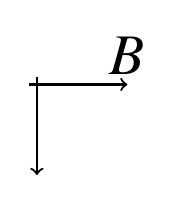
\begin{tikzpicture}
      \draw[->,thick] (-.1,0)--(1.15,0) node[above]
        {\huge $B$};
        % {Number of behaviors $B$};
      \draw[->,thick] (0,.1)--(0,-1.15) node[below]
        {\huge $\pilow$};
        % {Low payoff frequency $\pilow$};
	  \end{tikzpicture}~\\[-2em]

    \begin{minipage}{3.75in}
      \centering
      {\hspace{5.25em}\huge $B = 2$}
    \end{minipage}%
    \begin{minipage}{3.75in}
      \centering
      {\hspace{1.0em}\huge $B = 4$}
    \end{minipage}%
    \begin{minipage}{3.75in}
      \centering
      {\hspace{2.0em}\huge $B = 10$}
    \end{minipage}~\\

    \begin{minipage}{3.75in}
    \begin{rotate}{90}
      {\parbox{2.5in}{
          \centering
          \vspace{-2.5em} {\huge$ \pilow = 0.1$} \\
          {\begin{rotate}{-90}{\huge $\meansl$}\hspace{3em}\end{rotate}}
      }}
    \end{rotate}%
    \hspace{2em}
      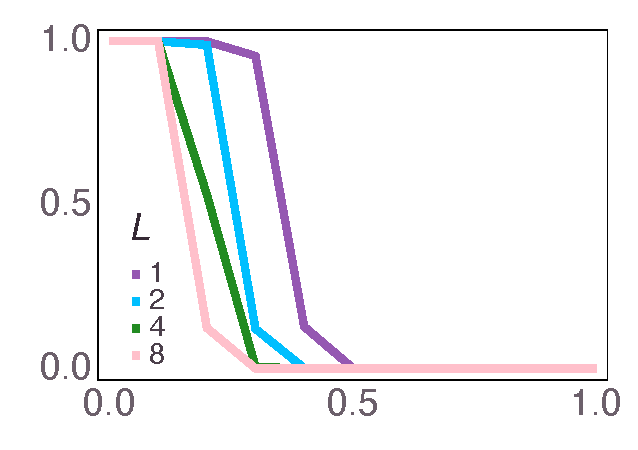
\includegraphics[width=\textwidth]{mean_social_learner_over_u_lowpayoff=0.1_nbehaviors=2.pdf}
    \end{minipage}\noindent\hspace{1.25em}
	\begin{minipage}{3.75in}%
      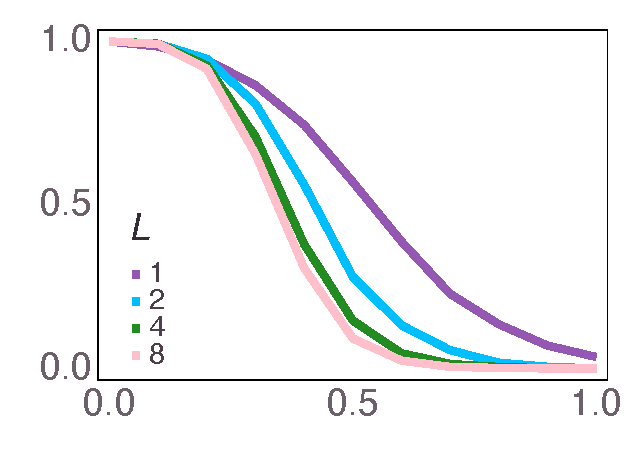
\includegraphics[width=\textwidth]{mean_social_learner_over_u_lowpayoff=0.1_nbehaviors=4.pdf}
    \end{minipage}\noindent
	\begin{minipage}{3.75in}%
      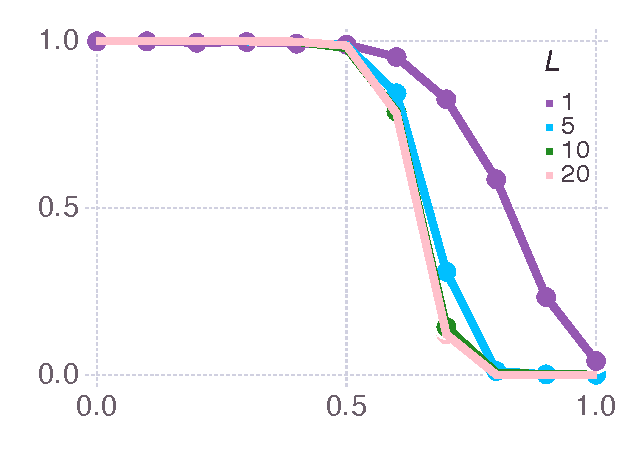
\includegraphics[width=\textwidth]{mean_social_learner_over_u_lowpayoff=0.1_nbehaviors=10.pdf}
    \end{minipage}~\\[0.5em]

    \begin{minipage}{3.75in}
    \begin{rotate}{90}
      {\parbox{2.5in}{
          \centering
          \vspace{-2.5em} {\huge$ \pilow = 0.45$} \\
          {\begin{rotate}{-90}{\huge $\meansl$}\hspace{3em}\end{rotate}}
      }}
    \end{rotate}%
    \hspace{2em}
      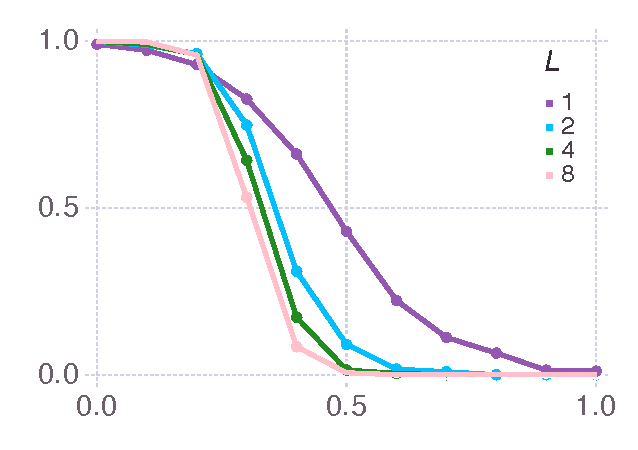
\includegraphics[width=\textwidth]{mean_social_learner_over_u_lowpayoff=0.45_nbehaviors=2.pdf}
	\end{minipage}\noindent\hspace{1.25em}
	\begin{minipage}{3.75in}%
      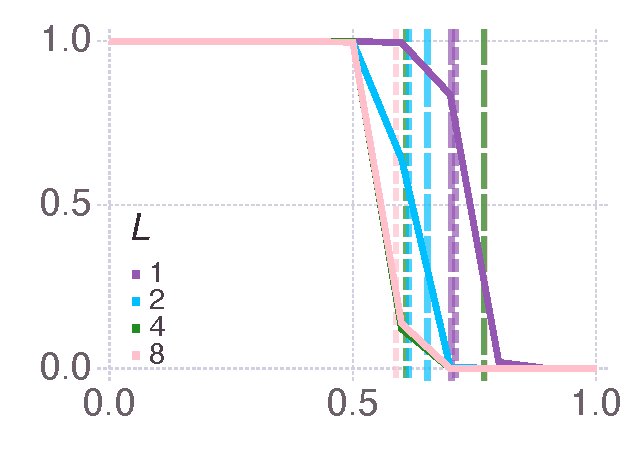
\includegraphics[width=\textwidth]{mean_social_learner_over_u_lowpayoff=0.45_nbehaviors=4.pdf}
    \end{minipage}\noindent
	\begin{minipage}{3.75in}%
      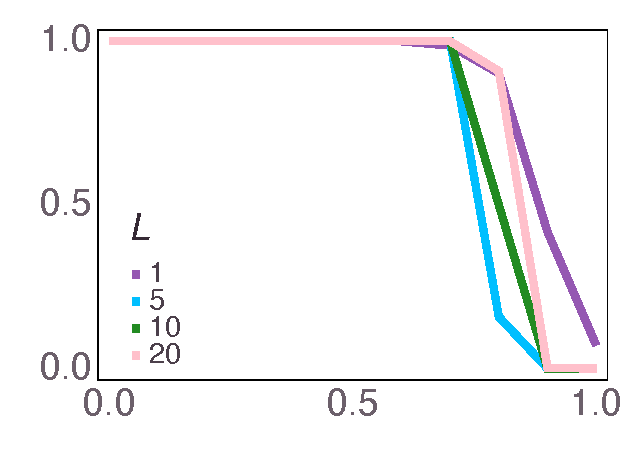
\includegraphics[width=\textwidth]{mean_social_learner_over_u_lowpayoff=0.45_nbehaviors=10.pdf}
    \end{minipage}~\\[0.5em]

    \begin{minipage}{3.75in}
    \begin{rotate}{90}
      {\parbox{2.5in}{
          \centering
          \vspace{-2.5em} {\huge$ \pilow = 0.8$} \\
          {\begin{rotate}{-90}{\huge $\meansl$}\hspace{3em}\end{rotate}}
      }}
    \end{rotate}%
    \hspace{2em}
      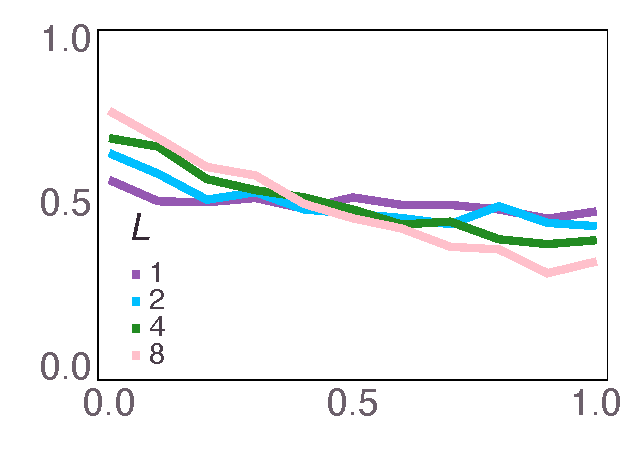
\includegraphics[width=\textwidth]{mean_social_learner_over_u_lowpayoff=0.8_nbehaviors=2.pdf}
        \\[-2.75em]
        \begin{center}
          {\hspace{3.25em} \huge $\quad u$}
      \end{center}
	  \end{minipage}\noindent\hspace{1.25em}
		\begin{minipage}{3.75in}%
		  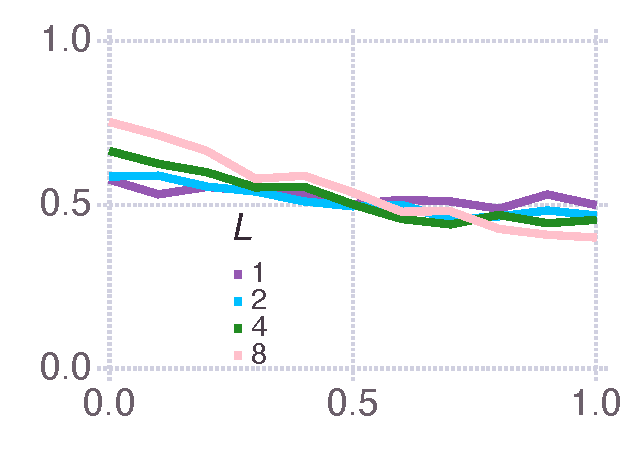
\includegraphics[width=\textwidth]{mean_social_learner_over_u_lowpayoff=0.8_nbehaviors=4.pdf}
		  \\[-2.75em]
	  \begin{center}
        {\huge $\quad u$}
      \end{center}
    \end{minipage}
	\begin{minipage}{3.75in}%
		  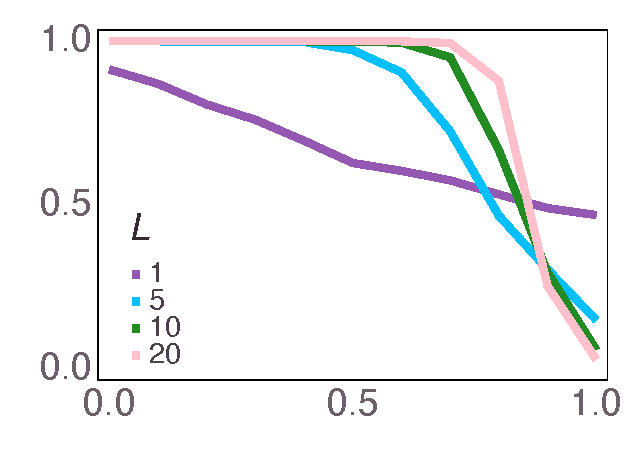
\includegraphics[width=\textwidth]{mean_social_learner_over_u_lowpayoff=0.8_nbehaviors=10.pdf}
		  \\[-2.75em]
	  \begin{center}
        {\huge $\quad u$}
      \end{center}
	\end{minipage}%
\end{document}


\section{Discussion}


\bibliographystyle{apacite}

\setlength{\bibleftmargin}{.125in}
\setlength{\bibindent}{-\bibleftmargin}

\bibliography{/Users/mt/workspace/Writing/library.bib}
% \bibliography{this.bib}

\end{document}
